\subsection{Umweltmodellierung}
\begin{figure}[ht]\centering 
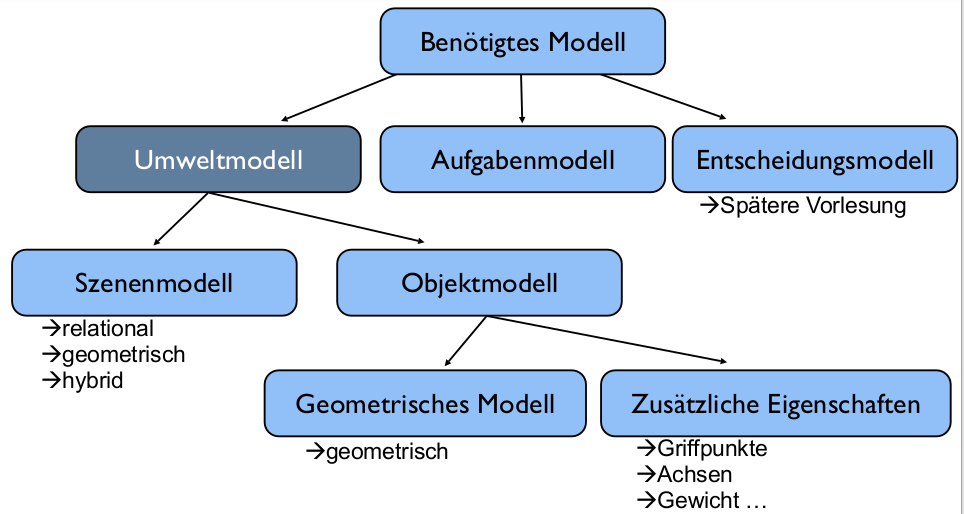
\includegraphics[width=0.6\linewidth]{figures/ch02_umweltmodell.png}
\caption{Umweltmodell}
\label{fig:ch02_um}
\end{figure}

%Keine Umlaute in labels!!!
\subsubsection{Objektmodell}
Die geometrische Beschreibung von Objekten beinhaltet:
\begin{itemize}
\setlength\itemsep{0em}
\item graphische Darstellung
\item Kollisionsberechnungen, Kontaktberechnung in Griffplanung, ...
\item physikalisch-dynamische Simulation der Effekte von Handlungen auf die Umwelt
\item geometriebezogene Bewegungsplanung
\end{itemize}
Es gibt drei Ansätze zur geometrischen Modellierung (\autoref{fig:obrepr}): 
\begin{enumerate}
\item Kantenmodelle
\item Flächenmodelle
\item Volumenmodelle
\end{enumerate}
\begin{figure}[h!]
	\centering
	\begin{subfigure}{.25\textwidth}
		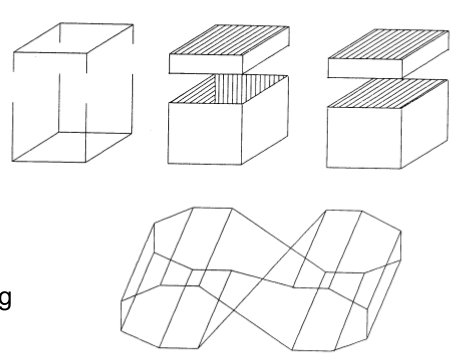
\includegraphics[width=\textwidth]{figures/ch02_kanten.png}
		\caption{}
	\end{subfigure}
	\begin{subfigure}{.25\textwidth}
		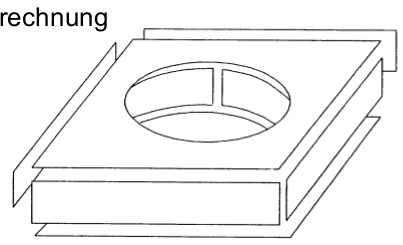
\includegraphics[width=\textwidth]{figures/ch02_flaechen.png}
		\caption{}
	\end{subfigure}
	\begin{subfigure}{.25\textwidth}
		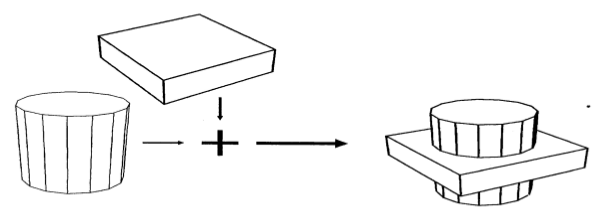
\includegraphics[width=\textwidth]{figures/ch02_volumen.png}
		\caption{}
	\end{subfigure}
	\caption{Objektrepr\"{a}sentation}
	\label{fig:obrepr}
\end{figure}
\paragraph*{Kanten}
Nur die Kanten werden gespeichert, d.h. Punkte und Verbindungen (Gerade, Polygonzug, Bezierkurve, ... ).
\begin{table}[hbt]
\centering
\begin{tabular}{|p{6.5cm}|p{6.5cm}|}
\hline
Vorteile & Nachteile\\
\hline
\vspace{-5mm}
\begin{itemize}
\setlength\itemsep{0em}
\item[+] einfache Daten
\item[+] wenige Daten
\end{itemize}
 &
 \vspace{-5mm}
\begin{itemize}
\setlength\itemsep{0em}
\item[-] Mehrdeutigkeiten (Abb. \ref{fig:obrepr}a unten)
\item[-] hoher Eingabeaufwand
\item[-] keine Kollisionsberechnung
\item[-] kein Schnitt
\end{itemize}\\
\hline
\end{tabular}
\caption{Zusammenfassung -- Kantenmodelle}
\label{tab:Kantenmod}
\end{table}\\ 
\paragraph*{Flächen}
Flächen können exakt modelliert werden, wenn sie \textcolor{red}{analytisch gegeben} sind (eine 3D Kugel beispielsweise durch $r = ||x-p||$, wobei $r$ der Radius und $p$ der Mittelpunkt ist).
\begin{table}[hbt]
\centering
\begin{tabular}{|p{6.5cm}|p{6.5cm}|}
\hline
Vorteile & Nachteile\\
\hline
\vspace{-5mm}
\begin{itemize}
\setlength\itemsep{0em}
\item[+] Geschlossene Darstellung (wenig Speicherbedarf)
\item[+] Analytische Darstellung erlaubt einfache Rechenverfahren (z.B.
Schnitt von Ebenen / Kugeln $\rightarrow$ schnelle Kollisionsberechnung)
\end{itemize}
 &
 \vspace{-5mm}
\begin{itemize}
\setlength\itemsep{0em}
\item[-] Wenige Flächen sind analytisch darstellbar
\end{itemize}\\
\hline
\end{tabular}
\caption{Flächen -- analytisch}
\label{tab:Flaechen-analyt}
\end{table}\\ 
Ansonsten werden sie \textcolor{red}{approximativ} durch Bildung einer großen Fläche aus einem Netz (\glqq Mesh\grqq ) von einfachen Einzelflächen (z.B. Dreiecke, Vierecke) modelliert.\\
\begin{table}[hbt]
\centering
\begin{tabular}{|p{6.5cm}|p{6.5cm}|}
\hline
Vorteile & Nachteile\\
\hline
\vspace{-5mm}
\begin{itemize}
\setlength\itemsep{0em}
\item[+] Definition sehr einfach
\item[+] einfache Algorithmen
\end{itemize}
 &
 \vspace{-5mm}
\begin{itemize}
\setlength\itemsep{0em}
\item[-] hoher Speicherbedarf
\item[-] hoher Rechenaufwand
\end{itemize}\\
\hline
\end{tabular}
\caption{Flächen -- approximativ}
\label{tab:Flaechen_approx}
\end{table}
\newpage
Hierbei werden Freiformflächen im einfachsten Fall durch \textbf{Dreiecksflächen} approximiert:
\begin{itemize}
\item[] Gegeben seien 3 Punkte im Raum $P_1 , P_2 , P_3$.
\item[] Damit hat die Fläche folgende Gleichung: $F(u,v)=u\cdot P_1 +v\cdot P_2 +(1-u-v)\cdot P_3$ mit $0 \leq u,v, u+v \leq 1$.
\begin{center}
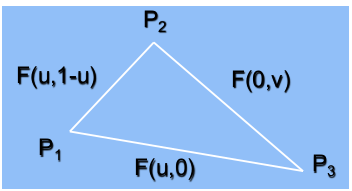
\includegraphics[width=.3\linewidth]{figures/ch02_dreieck.png}
\end{center}
\end{itemize}
Oder sie werden durch \textbf{Bilineare Viereckselemente / Pflaster} approximiert:
\begin{itemize}
\item[] Gegeben sind 4 Punkte im Raum $P_1 , P_2 , P_3, P_4$
\item[] Damit wird die Fläche definiert durch $F(u,v)=(1-u)(1-v) \cdot P_1 + (1-u)v \cdot P_2 + u(1-v) \cdot P_3 + uv \cdot P_4$ mit $0 \leq u \leq 1, 0 \leq v \leq 1$. 
\begin{center}
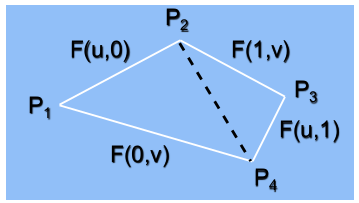
\includegraphics[width=.3\linewidth]{figures/ch02_pflaster.png}
\end{center}
\end{itemize}
\begin{table}[hbt]
\centering
\begin{tabular}{|p{6.5cm}|p{6.5cm}|}
\hline
Vorteile & Nachteile\\
\hline
\vspace{-5mm}
\begin{itemize}
\setlength\itemsep{0em}
\item[+] Flächenelemente können gekrümmt sein
$\rightarrow$ weniger Gitterpunkte bei gleich guter Approximation
\end{itemize}
 &
 \vspace{-5mm}
\begin{itemize}
\setlength\itemsep{0em}
\item[-] Rechnen mit gekrümmten Flächen ist aufwendig
\end{itemize}\\
\hline
\end{tabular}
\caption{Approximation durch Vierecke}
\label{tab:Viereck_approx}
\end{table}
Zudem können Flächen durch \textbf{Bezierflächen}, einer Erweiterung der Bezierkurven beschrieben werden:
\begin{itemize}
\item[] Gegeben ist ein Gitter von Führungspunkten $P_{ij}, 0 \leq i \leq N$ und $0 \leq j \leq M$.
\item[] Damit ist die Fläche beschrieben durch $F(u,v) = \sum_{i=0}^N \sum_{j=0}^M P_{ij} \cdot B_{i,N}(u) \cdot B_{j,M}(v)$\\
 mit $B_{i,N}(u) = (1-u)B_{i,N-1}(u)+uB_{i-1,N-1}(u)$\\
 und $B_{j,M}(v) = (1-v)B_{j,M-1}(v)+vB_{j-1,M-1}(v)$.
\item[] Die $B_{i,N}$ bzw. $B_{j,M}$ heißen auch Bernsteinpolynome.
\begin{center}
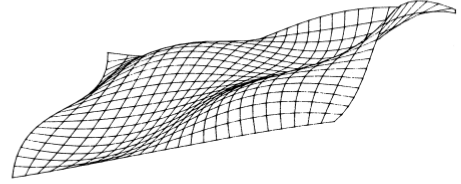
\includegraphics[width=.4\linewidth]{figures/ch02_bezier.png}
\end{center}
\end{itemize}
\begin{table}[hbt]
\centering
\begin{tabular}{|p{6.5cm}|p{6.5cm}|}
\hline
Vorteile & Nachteile\\
\hline
\vspace{-5mm}
\begin{itemize}
\setlength\itemsep{0em}
\item[+] effiziente Verfahren 
\item[+] entspricht dem Vorgehen während der Modellierung
\item[+] schnelle Kollisions- und Abstandsberechnung
\end{itemize}
 &
 \vspace{-5mm}
\begin{itemize}
\setlength\itemsep{0em}
\item[-] hoher Eingabeaufwand
\item[-] Darstellung aufwendig
\item[-] Problem bei Schnittoperationen
\item[-] Inkonsistenzen möglich
\end{itemize}\\
\hline
\end{tabular}
\caption{Zusammenfassung -- Flächenmodelle}
\label{tab:Flaechenmod}
\end{table}
\noindent
\paragraph*{Volumen} Vier verschiedene Arten von Volumenmodellen:\\ \\
\textbf{Parametrische Modelle}:\\
Grundkörper und topologische Operationen auf diesen (Schnitt, Vereinigung, ... ) werden abgespeichert. 
\begin{table}[hbt]
\centering
\begin{tabular}{|p{6.5cm}|p{6.5cm}|}
\hline
Vorteile & Nachteile\\
\hline
\vspace{-5mm}
\begin{itemize}
\setlength\itemsep{0em}
\item[+] eindeutige Objektbeschreibung 
\item[+] geringer Eingabeaufwand 
\item[+] Ergebnis von Operationen sind korrekte Objekte
\end{itemize}
 &
 \vspace{-5mm}
\begin{itemize}
\setlength\itemsep{0em}
\item[-] hoher Implementierungsaufwand
\item[-] Einbindung von Freiformflächen schwierig
\end{itemize}\\
\hline
\end{tabular}
\caption{Volumenmodelle -- parametrisch}
\label{tab:Volmod}
\end{table}\\ 
Die Objekte sind bereits vorhanden und können durch Angabe von Parametern angepaßt werden (Varianten).\\
Konsistenzprüfungen sind notwendig (\autoref{fig:kons})! \\
\begin{figure}[h!]
	\centering 
	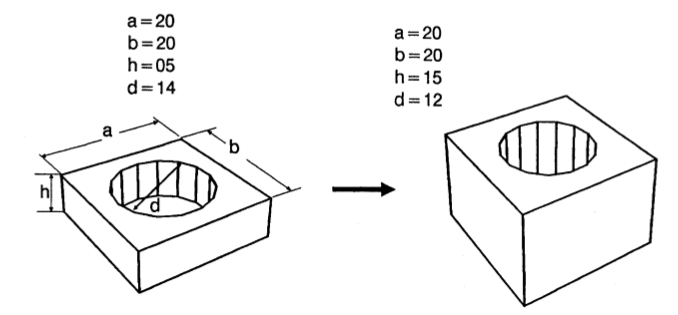
\includegraphics[width=0.3\linewidth]{figures/ch02_kons.png}
	\caption{Konsistenzprüfung: $d < min(a,b)$}
\label{fig:kons}
\end{figure}\\
\noindent
\textbf{Zellenzerlegung}:\\
 Objekte werden aus disjunkten Elementarzellen aufgebaut. Verwendung finden einfache geometrische Objekte z,B. Tetraeder, Quader, ...
Benutzt in der Strukturanalyse mit Finite-Elemente-Methoden (FEM).
\newpage
Diese Modelle können auf drei Arten umgesetzt werden:
\begin{enumerate}
\item Boundary Repräsentation
\item Constructive Solid Geometry (CSG)
\item Zellenbelegung
\end{enumerate}
\textbf{Boundary Repräsentation}: Hierarchische Darstellung eines Objektes durch begrenzende
Elemente, i.d.R. Kanten oder Flächen. \autoref{fig:brep} zeigt ein Beispiel.\\
\begin{figure}[h!]
	\centering 
	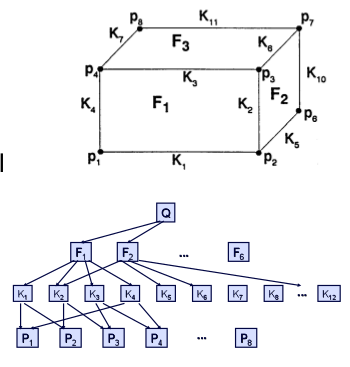
\includegraphics[width=0.3\linewidth]{figures/ch02_brep.png}
	\caption{Elemente eines Quaders im Flächenmodell: Quader $Q$, Flächen $F_i : i \in \{1,...,6\}$, Kanten $K_i : i \in \{1,...,12\}$, Ecken $P_i : i \in \{1,...,8\}$}
\label{fig:brep}
\end{figure}
Vorteile: aus der topologischen Struktur Information über z.B.:
\begin{itemize}
\item Welche Flächen gehören zum Objekt?
\item Welche Kanten gehören zur Fläche? $\rightarrow$ kantenbasierte Objekterkennung
\item Zu welchem Objekt gehört eine Fläche?
\item Zu welchem Objekt gehört eine Kante?
\item Welche Flächen stoßen aneinander?
\end{itemize}
\noindent
\textbf{Constructive Solid Geometry (CSG)}:
Es gibt eine Menge von einfachen Grundkörpern, die parametriert
werden können (\autoref{fig:csg}). 
\begin{figure}[h!]
	\centering
	\begin{subfigure}{.7\textwidth}
		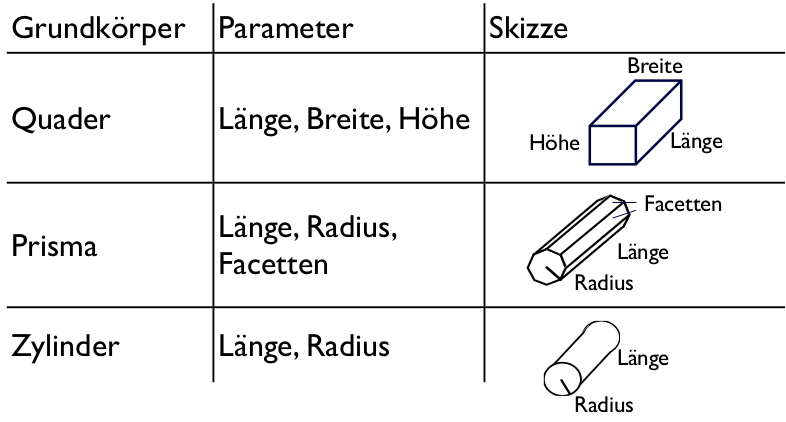
\includegraphics[width=\textwidth]{figures/ch02_csg.png}
	\end{subfigure}
	\begin{subfigure}{.7\textwidth}
		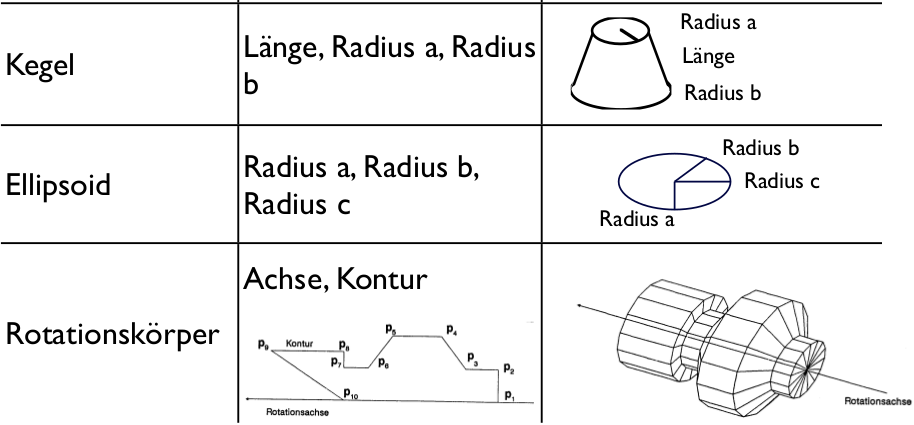
\includegraphics[width=\textwidth]{figures/ch02_csg1.png}
	\end{subfigure}
	\caption{Constructive Solid Geometry}
	\label{fig:csg}
\end{figure}
Auf ihnen sind verschiedene Operationen definiert, z.B.
\begin{table}[!hb]
\centering
\begin{tabular}{|p{6.5cm}|p{6.5cm}|}
\hline
 & Objekte $A$ 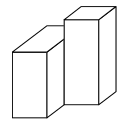
\includegraphics[width=.07\textwidth]{figures/ch02_a.png} \& $B$ 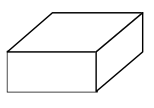
\includegraphics[width=.07\textwidth]{figures/ch02_b.png}\\
\hline
Vereinigung $A \cup B$ (Summe) & 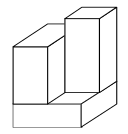
\includegraphics[width=.07\textwidth]{figures/ch02_ab.png}\\
\hline
Schnitt $A \cap B$ & 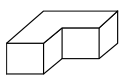
\includegraphics[width=.07\textwidth]{figures/ch02_ab1.png} \\
\hline
Differenz $A / B$ & 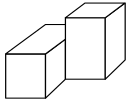
\includegraphics[width=.07\textwidth]{figures/ch02_ab2.png}\\
\hline
Sweep:
Ein Grundelement (u.U. eine Fläche) wird entlang einer Raumkurve
verschoben. Der durchdrungene Raum stellt das neue Objekt dar. & \\
\hline
\end{tabular}
\caption{CSG -- Operatoren}
\label{tab:csg_ops}
\end{table}\\ \\
\textbf{Zellenbelegung}:
Der Raum wird in mehrere Zellen unterteilt (i.d.R. 8 Zellen: \glqq Octree\grqq).
Wenn eine Zelle komplett vom Objekt belegt ist, als \glqq belegt\grqq{} markieren.
Wenn die Zelle nur teilweise belegt ist, dann wird auf diese Zelle das
Verfahren rekursiv angewendet. Ansonsten ist die Zelle leer.
Die Rekursion terminiert bei einer vorbestimmten minimalen Zellgröße.
Teilbelegte kleinste Zellen werden als belegt markiert. Siehe \autoref{zb}.
\begin{figure}[h!]
	\centering
	\begin{subfigure}{.45\textwidth}
		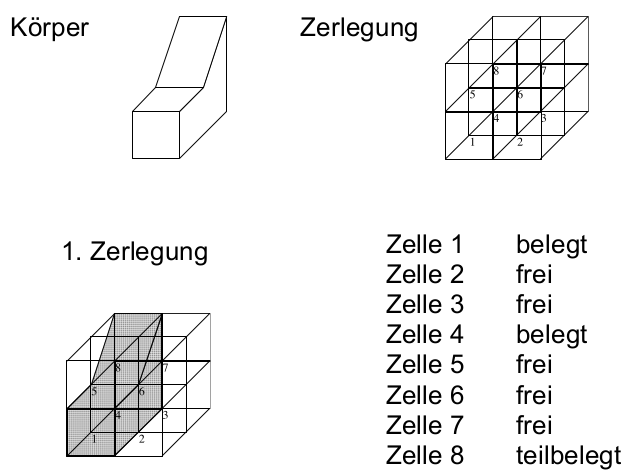
\includegraphics[width=\textwidth]{figures/ch02_zb.png}
	\end{subfigure}
	\begin{subfigure}{.45\textwidth}
		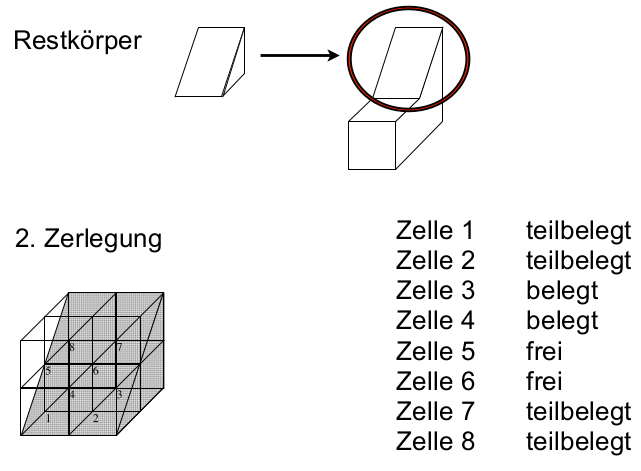
\includegraphics[width=\textwidth]{figures/ch02_zb1.png}
	\end{subfigure}
	\caption{Beispiel -- Zellenbelegung}
	\label{zb}
\end{figure}
\newpage
\subsection{Aufgabenmodellierung}
\begin{figure}[h!]\centering 
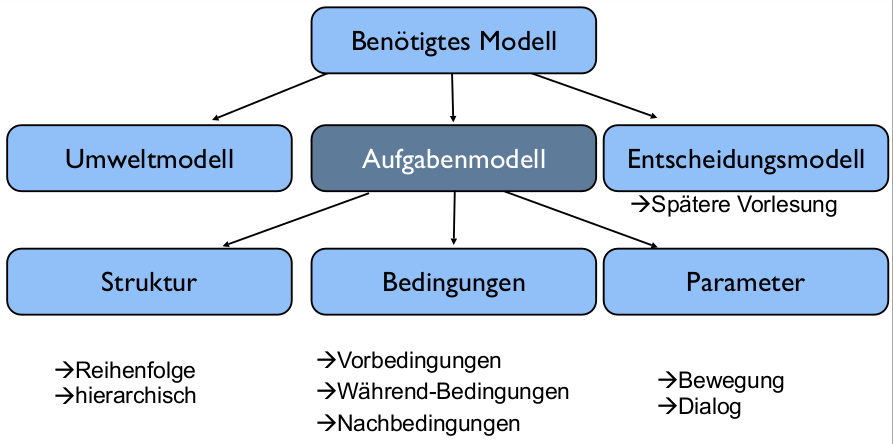
\includegraphics[width=0.6\linewidth]{figures/ch02_aufgabenmodell.png}
\caption{Aufgabenmodell}
\label{fig:ch02_am}
\end{figure}
%kognitive Lücke?
\begin{figure}[ht]\centering 
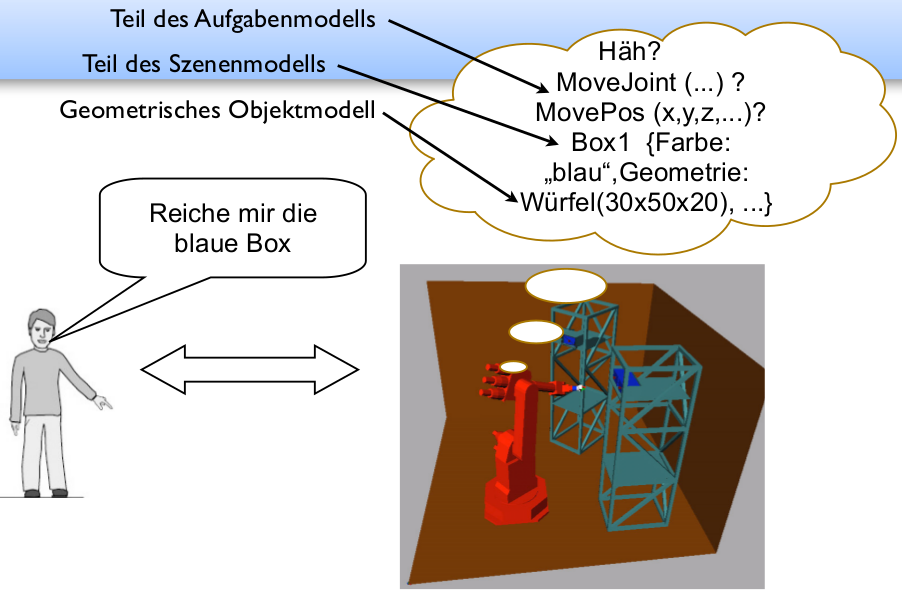
\includegraphics[width=0.6\linewidth]{figures/ch02_beispiel.png}
\caption{Beispiel}
\label{fig:ch02_bsp}
\end{figure}
\begin{figure}[h!]\centering 
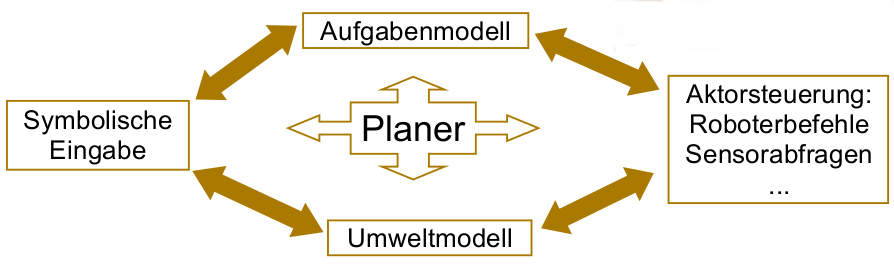
\includegraphics[width=0.6\linewidth]{figures/ch02_planer.png}
\caption{Einordnung des Aufgabenmodells}
\label{fig:ch02_ord}
\end{figure}
\textbf{Anforderungen an das Aufgabenmodell}:
\begin{itemize}
\item Erweiterbarkeit
\item Erklärbarkeit
\item Wiederverwendbarkeit
\item Integration des Wissens in ein Planungssystem
\end{itemize}
\newpage
\paragraph*{Symbolische Abstraktion}
Benutzer beschreibt die Aufgabe mit seinen Worten\\ (z.B. \glqq Bring mir Tee!\grqq) 
\begin{itemize}
\ita Abbildung: Erzeugung der Roboterbefehle über mehrere Stufen (vgl. \autoref{symbab})
\ita \glqq Fahre in die ‚Küche‘, greife ein Glas, fahre zurück und reiche mir den Becher.\grqq
\ita \glqq DriveTo(...), SearchObject(...), MoveArm(...), Grasp(Becher), MoveArm(...), DriveTo(...), MoveArm(...) ...!\grqq
\end{itemize}
\begin{figure}[h!]\centering 
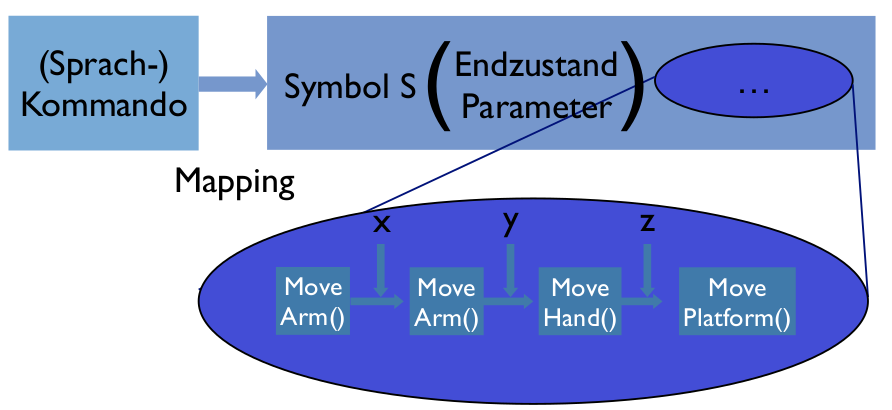
\includegraphics[width=0.6\linewidth]{figures/ch02_symbab.png}
\caption{Symbolische Abstraktion}
\label{symbab}
\end{figure}
\paragraph*{Modellierung der Reihenfolge von Operatoren/Symbolische Handlungsatome}
\begin{itemize}
\item In den gegebenen Beispielen wurden bereits implizit Handlungsatome angenommen
\item Die kleinsten auszuführenden Handlungseinheiten werden als
Elementaroperationen oder atomare Handlungen bezeichnet.
\item Komplexe Handlungen werden aus Elementaroperationen zusammengesetzt. Diese
können dazu üblicherweise parametriert werden.
\item Jeder Roboter besitzt eine endliche Menge an Elementaroperationen.
\end{itemize}
\paragraph*{Drei Ansätze für das Aufgabenmodell}
\begin{enumerate}
\item Sequentiell (\autoref{seq}): Festgelegte Folge von elementaren Aktionen 
\item Vorranggraph (\autoref{vorgra}): Darstellung der Abhängigkeiten
\item Hierarchisch (\autoref{hierar}): Abstraktion von Teilhandlungen
\end{enumerate}
\begin{figure}[h!]
	\centering
	\begin{subfigure}{.25\textwidth}
		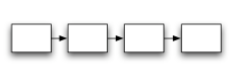
\includegraphics[width=\textwidth]{figures/ch02_ans.png}
		\caption{Sequentiell}
		\label{seq}
	\end{subfigure}
	\begin{subfigure}{.25\textwidth}
		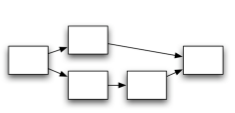
\includegraphics[width=\textwidth]{figures/ch02_ans1.png}
		\caption{Vorranggraph}
		\label{vorgra}
	\end{subfigure}
		\begin{subfigure}{.25\textwidth}
		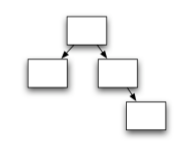
\includegraphics[width=\textwidth]{figures/ch02_ans2.png}
		\caption{Hierarchie}
		\label{hierar}
	\end{subfigure}
	\caption{Ansätze für das Aufgabenmodell}
	\label{ans}
\end{figure}
\newpage
\textbf{Sequentielle Handlungsbeschreibung}:
\begin{itemize}
\item Folge von (parametrierten) atomaren Handlungen
\item Eindeutig festgelegte Reihenfolge
\item Reihenfolge und Anordnung nicht unbedingt erklärbar (lesbar)
\item Bedingungen, Alternativen, etc. schlecht darstellbar
\item Sinnvoll für einfache Aufgaben oder sehr strukturierte Umgebungen (z.B. Leittechnik/Industrie)
\item Komplexe Handlungen: Rein sequentielle Beschreibungen nicht mächtig genug!
\item Ausführung sequentiell beschriebener Handlungen trivial
\item Linearer Handlungsfluss
\item Ausführung besteht aus: Anstoßen einer Elementarhandlung, evtl. Handlungsüberwachung und nach (erfolgreicher) Beendigung Übergang zur nächsten Elementarhandlung
\item Einfache Mechanismen zur Ausführung nötig!
\end{itemize}
\textbf{Vorranggraph}:
\begin{figure}[h!]
	\centering
	\begin{subfigure}{.45\textwidth}
		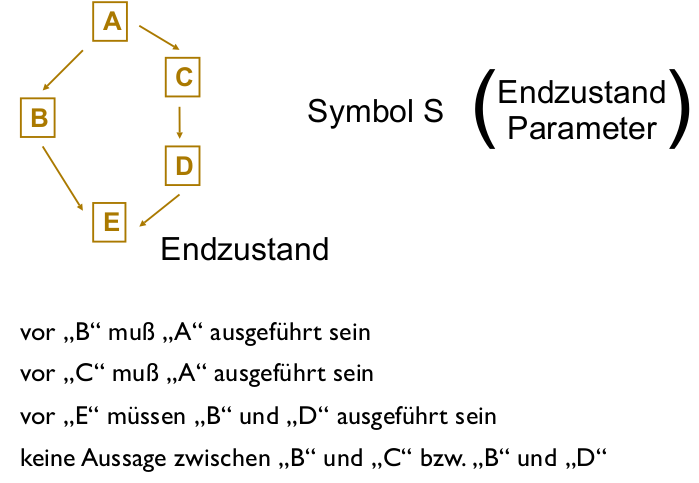
\includegraphics[width=\textwidth]{figures/ch02_vg-mod.png}
		\caption{Modellierung der Reihenfolge: Vorranggraph}
	\end{subfigure}
	\begin{subfigure}{.45\textwidth}
		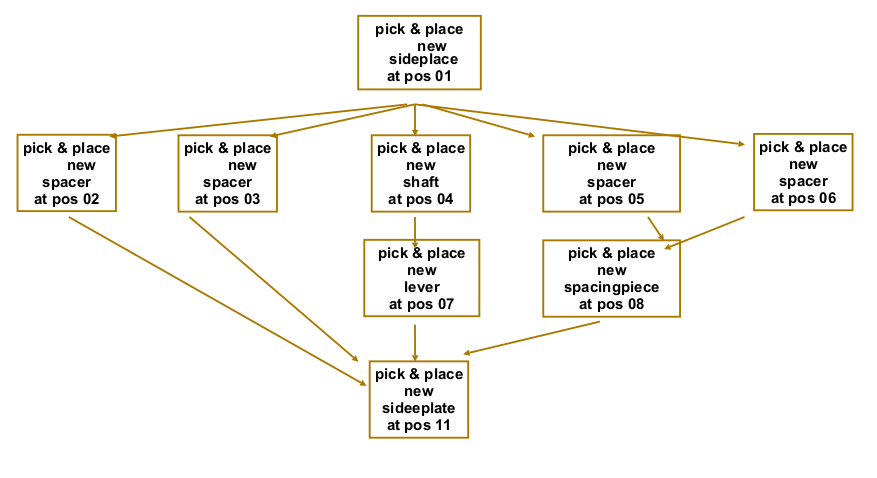
\includegraphics[width=\textwidth]{figures/ch02_vg-bsp.png}
		\caption{Beispiel: Vorranggraph des Cranfield-Benchmarks (simple Montage-Aufgabe)}
		\label{vg}
	\end{subfigure}
	\caption{Vorranggraph}
	\label{vg1}
\end{figure}
\begin{itemize}
\item Darstellung der Handlung in mehreren unabhängigen Teilzweigen
\item Üblicherweise: Serialisierung notwendig!
\begin{itemize}
\item Berechnung optimaler Operatorreihenfolgen
\item Freiheitsgrad zum Ausführungszeitpunkt
\item Serialisierung aufwendig ($\rightarrow$ Planungsverfahren, siehe spätere Vorlesungen)
\end{itemize}
\item Ausführung beinhaltet also:
\begin{itemize}
\item Serialisierung der Handlung nach gegebenen Kriterien
\item Ausführung der sequentiell beschriebenen Handlung
\end{itemize}
\item Mächtigere Handlungsbeschreibung benötigt auch mächtigere Verfahren bei der Ausführung!
\end{itemize}
\textbf{Hierarchisches Aufgabenmodell} (Abbildungen \ref{hier} und \ref{hiermod}):\\
Sowohl Aufgabenspezifikation als auch Aufgabenzerlegung/-teilung sind hierarchisch strukturiert. Die Abstraktion erfolgt nach Raum, Zeit, Objekten und Alternativen.
\begin{figure}[h!]\centering 
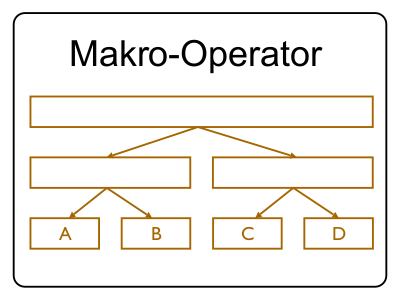
\includegraphics[width=0.3\linewidth]{figures/ch02_hier.png}
\caption{}
\label{hier}
\end{figure}\\
\begin{figure}[h!]
	\centering
	\begin{subfigure}{.45\textwidth}
		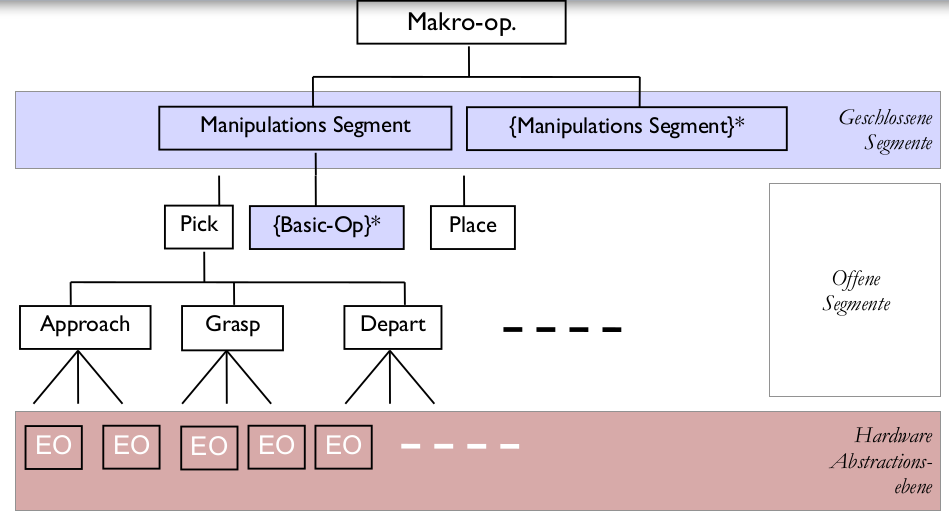
\includegraphics[width=\textwidth]{figures/ch02_hier1.png}
		\caption{Semantische hierarchische Repräsentation}
	\end{subfigure}
	\begin{subfigure}{.45\textwidth}
		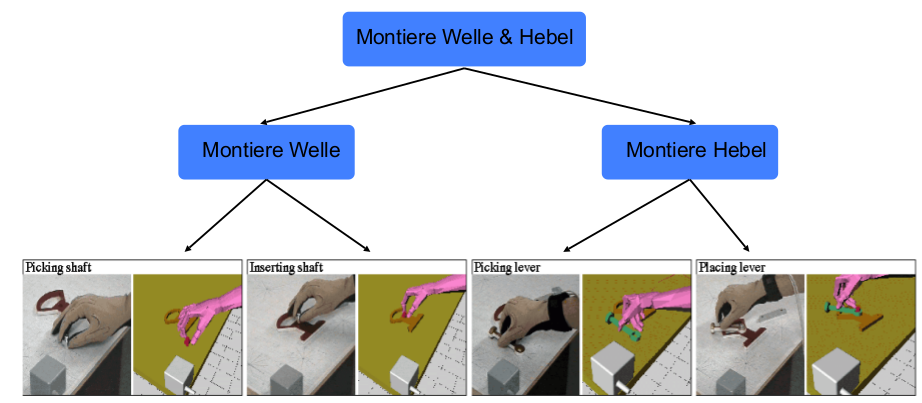
\includegraphics[width=\textwidth]{figures/ch02_hier2.png}
		\caption{Programmbeispiel: Montage von Welle und Hebel des Cranfield Benchmarks}
	\end{subfigure}
	\caption{Hierarchisches Aufgabenmodell}
	\label{hiermod}
\end{figure}
\paragraph*{Abstraktionsebenen im Aufgabenmodell}
Häufige Unterscheidung der in \autoref{abst} dargestellten semantischen Abstraktionsstufen. Diese benutzen symbolische Parameter.
\begin{itemize}
\ita Komplexität der Aufgabe beherrschbar
\ita Formalismen anwendbar
\end{itemize}
\begin{figure}[h!]\centering 
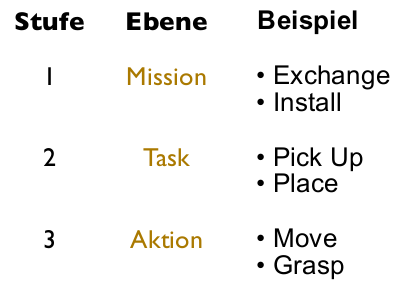
\includegraphics[width=0.3\linewidth]{figures/ch02_abst.png}
\caption{}
\label{abst}
\end{figure}
\textbf{Wahl der Abstraktionsebene}: Wie wird die Abstraktionsebene der Aktion gewählt, damit Aktionen von Roboter A auf Roboter B übertragen werden können?
\begin{itemize}
\item Aktion: Kleinste symbolische Einheit
\item Darunter: Regelungsebene
\item Abhängig von:
\begin{itemize}
\item Komplexität der Aufgabe
\item Grad der Kopplung einzelner Teilhandlungen
\item Hardware: Getrennt geregelte Komponenten werden üblicherweise auch mit getrennten Aktionen modelliert
\item Planungssystem/Beobachtungssystem
\end{itemize}
\item Grundsätzlich: Die Frage ist in der Forschung noch nicht eindeutig geklärt, immer noch ein Streitpunkt!
\end{itemize}
\textbf{Modellierung von Aktionen / Tasks}:\\
Ein \textcolor{red}{Operator} ist definiert durch $OP = (N, O, A, Par, K)$ mit
\begin{itemize}
\item $N$ = Name des Operators (eindeutig)
\item $O$ = Liste der beteiligten Objekte
\item $A$ = Auswahlbedingung
\item $Par$ = Liste der Parameter, z.B. Positionen, Kräfte, Beschleunigungen ...
\item $K$ = Körper des Operators:
\begin{itemize}
\item \textcolor{red}{\textbf{Aktion}/Elementaroperator}:\\ ausführbares Programm\\ $\Rightarrow$ Realisierung einfacher Fähigkeiten
\item \textcolor{red}{\textbf{Task}/Makro-Operator}:\\ besteht aus weiteren Operationen $K = K_1K_2...K_n$\\ $\Rightarrow$ Realisierung komplexer Aktionen
\end{itemize}
\end{itemize}
\textbf{Hierarchische Repräsentation -- Ausführung}:
\begin{itemize}
\item Im Aufgabenmodell ist die Serialisierung implizit gegeben
\begin{itemize}
\item Minimaler Aufwand zur Ausführung
\item Aber: Bei Parallelitäten von Teilhandlungen: Konflikte möglich!
\end{itemize}
\item Ausführung beinhaltet also:
\begin{itemize}
\item Überprüfung auf Konflikte
\item Gegebenenfalls Serialisierung/Lösen der Konflikte
\item Ausführung der resultierenden Operatorsequenz
\end{itemize}
\item Vorteil: Zusammengesetzte (Teil-)Programme können wiederverwendet werden
\item Repräsentation gut \glqq lesbar\grqq{} (verständlich, erklärbar)
\end{itemize}
\textbf{Anwendung hierarchischer Handlungsbeschreibung in der Realität  \\-- Flexible Programme}:\\
Symbolische Abstraktionsebene zur Roboterprogrammierung
\begin{itemize}
\item Hierarchische Handlungsbeschreibung
\item Erklärbar, verständlich, intuitiv
\item Wiederverwendbarkeit
\item Parametrierbar
\item Unterstützt: Bedingungen, Verzweigungen, Ressourcenverwaltung, Parallelität
\item Aufbau flexibler Programme:
\begin{itemize}
\item Repräsentation des Handlungswissens als Baumstruktur
\item Parametrierbare Aktionsbeschreibung
\item Blätter entsprechen Roboteraktionen
\item Abarbeitung entsprechend einer Tiefensuche
\item Instantiierung der Kinder zur Laufzeit (Expansion des Baums)
\item Auswahl des geeignetsten Kandidaten beim expandieren
\item Parallele Ausführung mehrerer Kinder möglich
\end{itemize}
\end{itemize}
\paragraph*{Validierung der Modelle: Simulation oder Graphische Animation}
\begin{enumerate}
\item \textbf{Simulation der Komponenten}: Validierung anhand gegebener Einschränkungen (Kollisionen, Erreichbarkeit, Optimalitätskriterien: Weg, Zeit, Energie, ...)
\begin{itemize}
\ita Für die Simulation von Effekten durch Manipulatoren wird die Physiksimulation verwendet: Masse, Reibung, Kräfte, Gelenke
\end{itemize}
\item \textbf{Graphische Animation}: Der Anwender überprüft visuell die erstellten Modelle
\begin{itemize}
\ita Wenn die Robotersimulationen ergeben, dass die Zielstellung angefahren werden kann, wird die Bewegung in einer Animation graphisch dargestellt.
\end{itemize}
\end{enumerate}

\paragraph*{Aufgabenmodell -- Zusammenfassung und Diskussion}\phantom\newline
\textbf{Zusammenfassung}:
\begin{itemize}
\item Aufgabenmodell basiert auf elementaren Operationen
\item Oft dreischichtiger Ansatz: Aktion, Task, Mission
\item Verknüpfung der elementaren Operationen zu komplexen Aufgaben:
\begin{itemize}
\item Sequentiell
\item Vorranggraph
\item  Hierarchisch
\item (Kontrollstrukturen)
\end{itemize}
\item Problem: Validierung der Programme
\begin{itemize}
\item Simulation
\item Animation und Validierung durch den Menschen
\end{itemize}
\end{itemize}

\textbf{Diskussion}:
\begin{itemize}
\item Mobile Plattform ohne Sensorik (z.B. Roomba)
\begin{itemize}
\item Aufgabenmodell?
\item Umweltmodell?
\end{itemize}
\item Mobile Plattform mit Differentialantrieb und Sensorik zur Lokalisation (z.B. Transportaufgaben)
\begin{itemize}
\item Aufgabenmodell?
\item Umweltmodell?
\end{itemize}
\item Serviceroboter mit mobiler Plattform, Manipulator, Mehrfingergreifer, komplexe Sensorik\begin{itemize}
\item Aufgabenmodell?
\item Umweltmodell?
\end{itemize}
\item Wo kommt jeweils das Aufgabenwissen dieser Systeme her?
\end{itemize}